\documentclass[12pt]{article}

% Language setting
\usepackage[utf8]{inputenc}
\usepackage[bulgarian]{babel}

% --------------------- Packages  --------------------
% Use biblatex
\usepackage{biblatex}
\addbibresource{bibliography.bib}
% Table thickness
\usepackage{ctable}
% Equations: SI units
\usepackage{siunitx}
% Approximately equal
\usepackage{amssymb}
% degrees symbol
\usepackage{gensymb}
% warning box
\usepackage{pifont,mdframed}

\newenvironment{warning}
  {\par\begin{mdframed}[linewidth=2pt, linecolor=white]%
    \begin{list}{}{\leftmargin=1cm
                   \labelwidth=\leftmargin}\item[\Large\ding{43}]}
  {\end{list}\end{mdframed}\par}

% --------------------- Title  --------------------
\addbibresource{bibliography.bib}

\begin{document}

% Anfang der Titelseite________________________________________________________________________________
\begin{titlepage}
	\flushleft
% 	\begin{center}
	%{\scshape\Large Werkstoffe III \hspace{2.5cm} Laborbericht \hspace{2.5cm}HS 2022 \par}
	{\scshape\Large Протокол VIII \hspace{1.5cm} Механика - практикум\par}
	\vspace{5cm}
	{\huge\bfseries Реверсионно махало\par}
	\vspace{1cm}
	{\LARGE\bfseries Лабораторно упражнение №8\par}
	\vspace{5cm}
    % {\LARGE\bfseries Физически Факлутет към Софийски Университет ``Св. Климент Охридски \par}
    {\LARGE\bfseries Виолета Кабаджова, \par}
%   {\LARGE\bfseries Group: X\par}
    {\large\bfseries ККТФ, фак. номер: 3PH0600026\par}
	\vspace{1cm}
	
	{\large Физически Факултет, 
	
	Софийски Университет "Св. Климент Охридски"
	
	15 ноември 2022 г.\par}
	
\end{titlepage}

\section{Теоритична част}\label{sec:theoretical-part}
% \begin{figure}
%     \centering
%     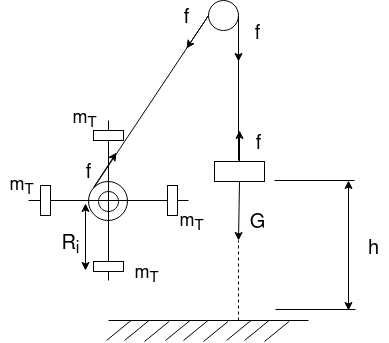
\includegraphics[width=0.5\textwidth]{images/oberbeck.drawio.png}
%     \caption{Схема на уред на Обербек}
%     \label{fig:setup}
% \end{figure}

Математично махало е физичен модел, при който материална точка е окачена на неразтеглива и безтегловна нишка с дължина l. При малки ъгли на отклонение от равновесното положение периодът му се определя по формула \ref{eq:period-math-pendulum}, където g е земното ускорение.

\begin{equation}\label{eq:period-math-pendulum}
    T_M = 2 \pi \sqrt{\frac{l}{g}}
\end{equation}

Физичното махало от своя страна е всяко твърдо тяло, което под действие на момента на силата на тежестта може да извършва трептения около неподвижна хоризонтална ос, която не минава през центъра на масите му. Движението на физично махало се описва чрез основното уравнение на динамиката на въртеливите движения - ур. \ref{eq:main-eq-rotation}, в което $I$ - инерчен момент спрямо оста на въртене Oz, $\beta_z$ - ъглово ускорение. Периодът на трептене за физично махало може да бъде определен посредством формула \ref{eq:main-physical-pendulum}, където $I$ е инечрният момент спрямо оста, $D = mgd $ - дирекционният момент на физичното махало 

\begin{equation}\label{eq:main-eq-rotation}
    M_z = I\beta_z
\end{equation}

\begin{equation}\label{eq:main-physical-pendulum}
    T_\Phi = 2\pi \sqrt{\frac{I}{D}} 
\end{equation}

От формули \ref{eq:period-math-pendulum} и \ref{eq:main-physical-pendulum} приравнявайки двата периода можем да открием физично махало, чието поведение ще бъде като това на математично. Тогава дължината $l = \frac{I}{md} = L_p$ от тези формули ще се нарича приведена (редуцирана) дължина на физичното махало ($L_p > d$). 

Точката, получена от нанасянето на редуцираната дължина $L_p$ от точката на окачване на махалото по ос, минаваща през центъра на масите, се нарича център на люлеене. Махало, при което точката на окачване и точката на люлеене са взаимнозаменяеми, се нарича реверсионно махало. То се използва за измерване на земното ускорение, тъй като редуцираната му дължина може да бъде пряко измерена и оттам да се заместят съответните стойности във формула \ref{eq:period-math-pendulum}.


\section{Експериментална част}
\begin{figure}
    \centering
    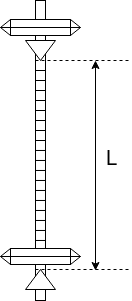
\includegraphics[width=0.2\textwidth]{images/katers-pendulum.drawio.png}
    \caption{Схема на реверсионно махало}
    \label{fig:setup}
\end{figure}

\subsection{Експериментална установка} 
На фиг. \ref{fig:setup} е представена схема на реверсионно махало, състоящо се от разграфена метална пръчка, две неподвижини призми, които фиксират дължината L, една неподвижна тежест, разположена зад една от призмите, и една подвижна, чрез която променямe центъра на масите на махалото и оттам инерчния и дирекционния момент. Чрез преместване на подвижната тежест търсим редуцираната дължина на физичното махало, след откриването на която можем да измерим земното ускорение.

\subsection{Задача: Измерване на земното ускорение g}
Експериментът се състои в това да преместим подвижната тежест от крайно горно положение до крайно долно, като на всяко деление на скалата броим по десет периода. След достигане на крайно долно положение, обръщаме реверсионното махало на 180\degree от началното положение и повтаряме.  

Направените измервания записваме в таблица \ref{tbl:meas} и налагаме на две графики на фиг. \ref{fig:results}. Тези графики се пресичат в две точки (измервания N=4 и N=42), като взимаме средноаритметичната на стойностите им, за да определим периода $T_\Phi = \frac{1}{10} \frac{T_1 + T_2}{2} = 1.335$ s. Забелязваме, че едната от точките на пресичане е именно на последното измерване, затова взимаме и цялата дължина на махалото, измерена след завъртането на махалото, за да се направят втората половина от измерванията, $L_p = 44.6$ cm. Заместваме стойностите във формула \ref{eq:g}, която следва от формула \ref{eq:period-math-pendulum}, и получаваме стойността на земното ускорение $g = 9.88 \pm 0.08$ m/s$^2$. 

\begin{equation}\label{eq:g}
    g = \frac{4\pi^2L_p}{T_\Phi^2}
\end{equation}

\begin{figure}
    \centering
    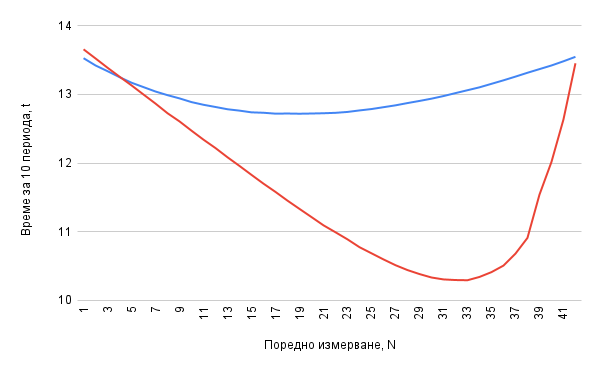
\includegraphics[width=1\textwidth]{images/chart.png}
    \caption{Графична зависимост на периода на махалото от положението на подвижната ос}
    \label{fig:results}
\end{figure}

\begin{table}[h]
\begin{center}
\begin{tabular}{|l|l|l|} \hline
N &t_{i1}, [s] &t_{i2}, [s] \\\hline
1 &1.3525 &1.3654 \\\hline
2 &1.3419 &1.3521 \\\hline
3 &1.3336 &1.3386 \\\hline
4 &1.3249 &1.3256 \\\hline
5 &1.3168 &1.3129 \\\hline
6 &1.3104 &1.2996 \\\hline
7 &1.304 &1.2864 \\\hline
8 &1.2987 &1.2724 \\\hline
9 &1.294 &1.2605 \\\hline
10 &1.2886 &1.247 \\\hline
11 &1.2847 &1.2339 \\\hline
12 &1.2815 &1.2217 \\\hline
13 &1.2782 &1.2083 \\\hline
14 &1.2762 &1.1957 \\\hline
15 &1.2737 &1.1827 \\\hline
16 &1.2731 &1.1699 \\\hline
17 &1.2718 &1.1579 \\\hline
18 &1.272 &1.1452 \\\hline
19 &1.2717 &1.1332 \\\hline
20 &1.272 &1.1213 \\\hline
21 &1.2724 &1.1093 \\\hline
\end{tabular}
\hspace{2cm}
\begin{tabular}{|l|l|l|} \hline
22 &1.273 &1.0992 \\\hline
23 &1.2743 &1.0889 \\\hline
24 &1.2765 &1.0775 \\\hline
25 &1.2785 &1.0686 \\\hline
26 &1.2812 &1.0597 \\\hline
27 &1.2839 &1.0513 \\\hline
28 &1.2872 &1.0442 \\\hline
29 &1.2903 &1.0384 \\\hline
30 &1.2936 &1.0334 \\\hline
31 &1.2974 &1.0306 \\\hline
32 &1.3017 &1.0297 \\\hline
33 &1.3059 &1.0294 \\\hline
34 &1.3101 &1.0342 \\\hline
35 &1.3152 &1.0412 \\\hline
36 &1.3203 &1.0507 \\\hline
37 &1.3257 &1.0681 \\\hline
38 &1.3313 &1.091 \\\hline
39 &1.3366 &1.1539 \\\hline
40 &1.3419 &1.2015 \\\hline
41 &1.348 &1.2633 \\\hline
42 &1.3545 &1.3451 \\\hline
\end{tabular}
\caption{\label{tbl:meas}Измеване на времето за 10 периода на махалото в различни части на скалата преди обръщането на махалото ($t_{i1}$) и след обръщането му ($t_{i2}$).}
\end{center}
\end{table}

\end{document}
